\documentclass{article}
\usepackage{graphicx} % Required for inserting images
\usepackage{float}
\usepackage[section]{placeins}

\title{Assignment 1}
\date{October 8, 2023}
\author{
  Ravi Raghavan\\
  \texttt{rr1133}
  \and
  Michelle Han\\
  \texttt{mmh255}
}

\begin{document}
\maketitle
\section{Generate, visualize and store 2D polygonal scenes}

\subsection{Example Maps}
The density of the maps was controlled by the amount of polygons in relation to the radii. Maps with greater radii (Fig. 1) required less polygons to fill the space compared to maps with smaller radii (Fig. 2). The shape of the polygons was controlled by the number of vertices. Maps with higher number of vertices resulted in polygons that were more round in appearance (Fig. 3 and 4). Maps with a lower amount of vertices appeared more sharp (Fig. 1 and 2). The four maps generated using \textit{constructScene} and their corresponding parameters:
\subsubsection{Big and Dense Polygons (see Fig. 1)}
Number of Polygons: 10
\\Minimum Number of Vertices: 4\space\space\space\space\space\space Maximum Number of Vertices: 6
\\Minimum Radius: 0.3\space\space\space\space\space\space\space\space\space\space\space \space\space\space\space\space\space \space\space\space Maximum Radius: 0.4
\subsubsection{Small and Dense Polygons (see Fig. 2)}
Number of Polygons: 30 
\\Minimum Number of Vertices: 4 \space\space\space\space\space\space Maximum Number of Vertices: 6
\\Minimum Radius: 0.1 \space\space\space\space\space\space\space\space\space\space\space \space\space\space\space\space\space \space\space\space Maximum Radius: 0.2
\subsubsection{Small and Sparse Polygons (see Fig. 3)}
Number of Polygons: 5
\\Minimum Number of Vertices: 15 \space\space\space\space\space\space Maximum Number of Vertices: 20
\\Minimum Radius: 0.05 \space\space\space\space\space\space\space\space\space\space\space \space\space\space\space\space\space \space\space\space Maximum Radius: 0.1
\subsubsection{Big and Sparse Polygons (see Fig. 4)}
Number of Polygons: 3
\\Minimum Number of Vertices: 5 \space\space\space\space\space\space Maximum Number of Vertices: 15 
\\Minimum Radius: 0.4 \space\space\space\space\space\space\space\space\space\space\space \space\space\space\space\space\space \space\space\space Maximum Radius: 0.6
\begin{figure}[htbp]
  \centering
  \begin{minipage}{0.45\textwidth}
    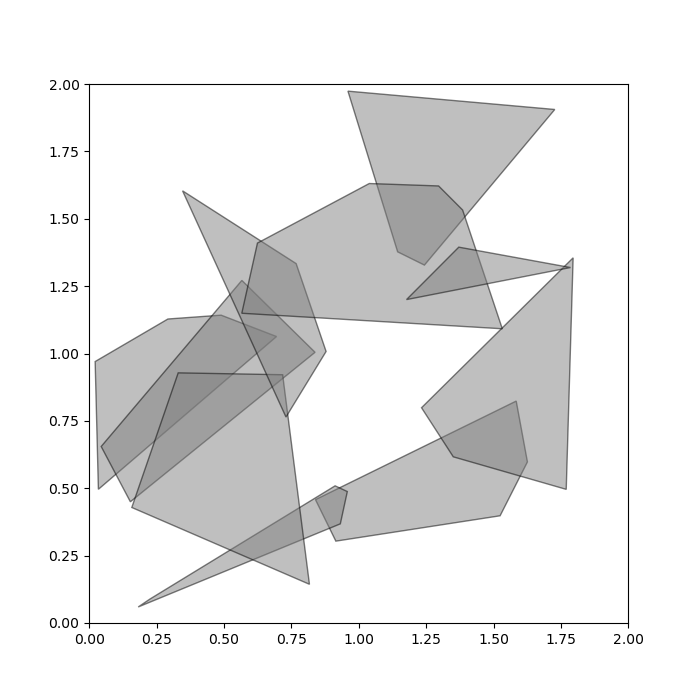
\includegraphics[width=\linewidth]{part1_big_dense.png}
    \caption{Big and dense polygons}
  \end{minipage}\hfill
  \begin{minipage}{0.45\textwidth}
    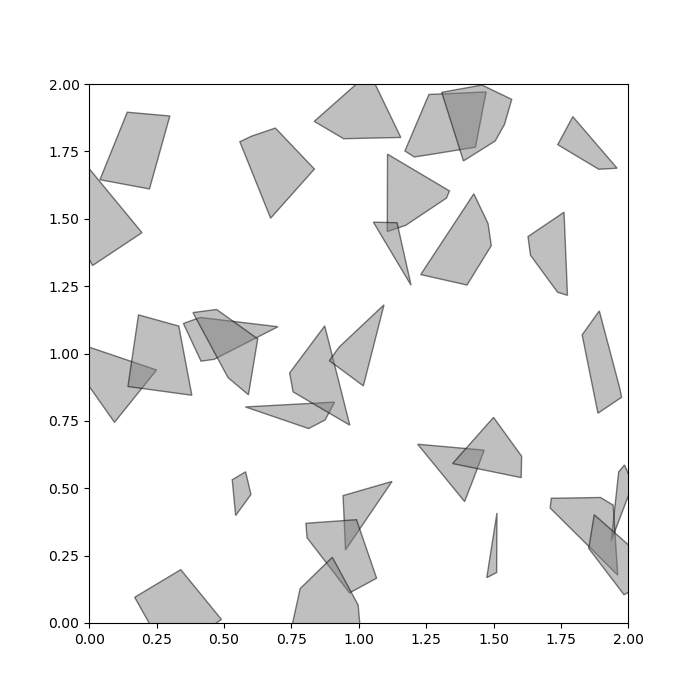
\includegraphics[width=\linewidth]{part1_small_dense.png}
    \caption{Small and dense polygons}
  \end{minipage}
  \begin{minipage}{0.45\textwidth}
    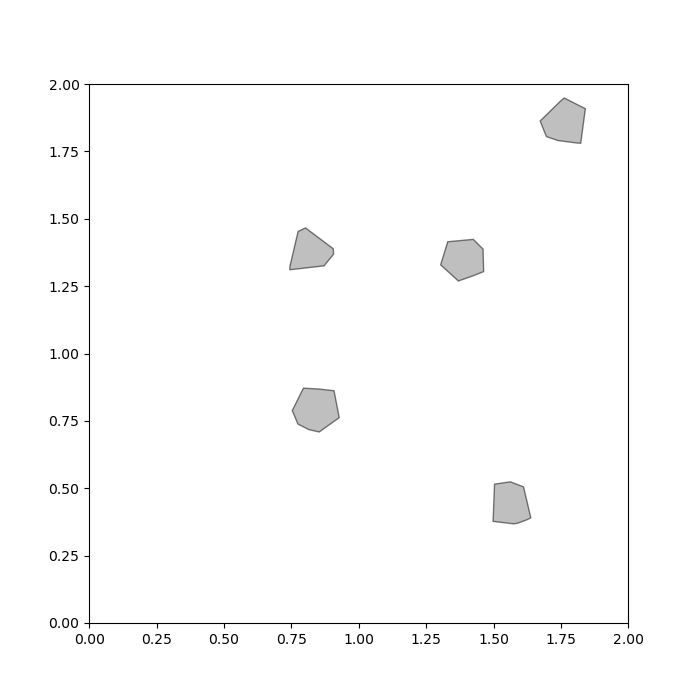
\includegraphics[width=\linewidth]{part1_small_sparse.png}
    \caption{Small and sparse polygons}
  \end{minipage}\hfill
  \begin{minipage}{0.45\textwidth}
    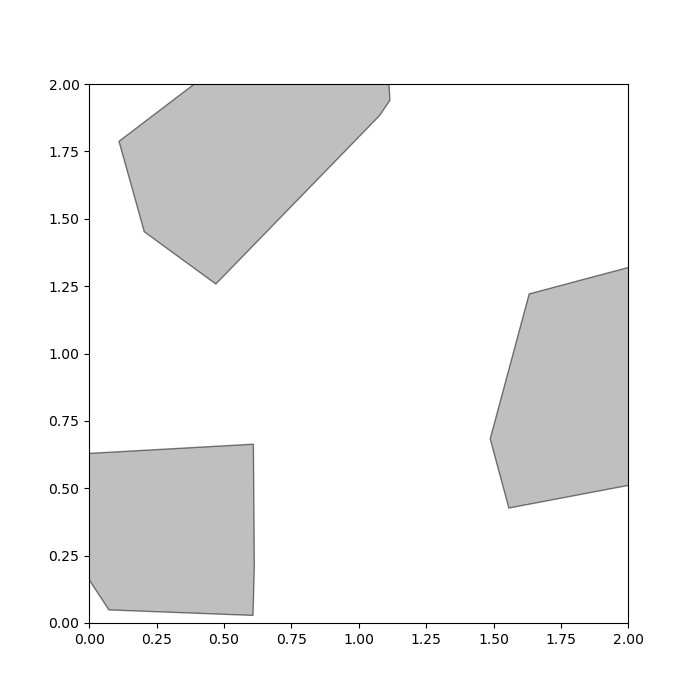
\includegraphics[width=\linewidth]{part1_sparse_big.png}
    \caption{Big and sparse polygons}
  \end{minipage}
\end{figure}

\subsection{Convex Polygon Letters}
\begin{figure}[H]
  \centering
  \begin{minipage}{0.45\textwidth}
    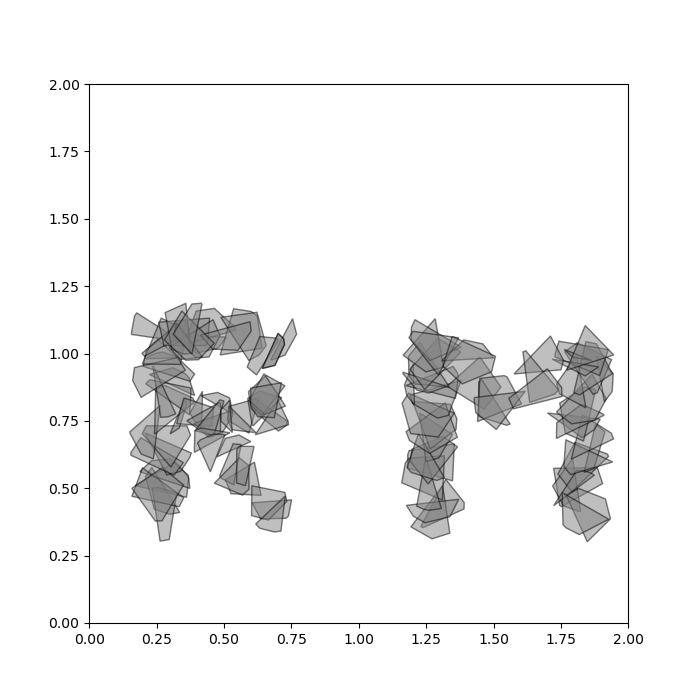
\includegraphics[width=\linewidth]{part1_letters.png}
    \caption{R and M generated using convex polygons}
  \end{minipage}\hfill
\end{figure}
\subsection{Convex Polygon Strategy}
In order to generate convex polygons, the strategy outlined in the write up was followed.
\subsubsection{Polygon Rotation}
A randomly sampled vertex (\textit{xcenter , ycenter}) was created inside the 2mx2m map. Using this vertex as the center, the minimum radius \textit{rmin} was used to generate a circle of radius \textit{rmin}. An angle, $\theta$, is sampled from [0°,360°]. A vertex is calculated by: 
    \[x = xcenter + r*cos(\theta)\]
    \[y = ycenter + r*sin(\theta)\]
 The expressions determine where the vertice falls on the circle. This is repeated N times to get N vertices from [\textit{nmin, nmax}]. The placement of the vertices along the circumference of a circle of radius \textit{rmin} allows for the polygon to be rotated.
\subsubsection{Extrude Vertices}
To extrude a vertex, a radius \textit{r} is sampled from [0, maximum vertices - minimum vertices]. The range [0, maximum vertices - minimum vertices] allows for a vertex to lie outside of the polygon's minimum radius. It allows for the circle that the new vertex lies on to be equal to or greater than radius \textit{rmin}. The new position of the vertex is calculated by: 
    \[new x = x + r*cos(\theta)\]
    \[new y = y + r*sin(\theta)\]
This process is repeated for all the vertices in the polygon. 
\subsubsection{Convexity of Polygons}
To determine the convexity of a generated polygon, the \textit{ConvexHull} function was used. The \textit{makeConvex} function takes a polygon and applies \textit{ConvexHull} to it. The result is the indices of vertices that form a convex polygon in counterclockwise order. This is stored in \textit{hull}. The indices in \textit{hull} are used to extract the vertices of the polygon that form a convex polygon into \textit{vertices}. Another vertex, the first one, is appended to \textit{vertices} so that the polygon is closed. \textit{convexPolygons} is ordered in counterclockwise order. If the given polygon is already convex, then convexPolygons will receive the same amount of vertices as the original polygon. 

\section{2D collision checking for convex polygons}
\subsection{Implementation Details} 
To implement the collision checking approach, I had two methods. The first method was a naive method and the second method was an optimized method. I implemented this collision checking approach two ways so that I could do a comparison between both implementations to see how the optimized approach fares with respect to the overall runtime. 

\subsubsection{Naive Approach}
The naive approach I implemented was rather simplistic. The first thing I did was to check all pairs of line segments between the two polygons for collisions. Then, I checked to see if any of the vertices of one polygon are inside the other. If I had cases where there was either an intersection between one line segment from one polygon and a line segment from the other polygon or one vertex of one polygon was inside the other polygon, then I would return True to indicate that we had a collision. If I did not encounter either of these two cases, I would return False to indicate that there is NO collision.  

\subsubsection{Optimized Approach}
To implement the optimized approach, my methodology can be broken down into two major portions. Let's say we are trying to detect if Polygon P and Q collide. The first thing I did was to construct bounding boxes around each polygon. Essentially, a bounding box for a polygon is akin to drawing a rectangle around the polygon that covers all its corners \newline 

Once the bounding boxes are constructed, when checking for collision, the first thing I check to see is if the bounding boxes for P and Q intersect. If no intersection is detected, I simply return False to indicate that there is NO collision. \newline 

However, if there is a collision detected between the bounding boxes of P and Q, I need to verify this collision. To do this verification, I use the Separating Axis Theorem(SAT). \newline 

Essentially, the main principle behind the Separating Axis Theorem is as follows. If a line/axis exists such that the projections of two polygons onto this line don't overlap, then the polygons don't collide. \newline 

For each edge of both polygons, I computed the normal vector to that edge. Then, I projected each polygon onto that normal vector. If there was a gap in the projections(i.e. there was no overlap in the projections), then I could conclude that there was NO intersection between the two polygons. Else, if there was no such gap, then there was an intersection between the two polygons. 

\subsubsection{Alternative Optimized Approach}
I implemented a third optimized approach which was to use Minkowski Differences to detect collisions. Given two polygons $P$ and $Q$, they collide iff their Minkowski Difference contains the origin. \newline 

To compute the Minkowski Difference of polygons P and Q, the first thing I did was multiply the vertices of Polygon Q to get $-Q$. Then, I would essentially compute the Minkowski Sum of $P$ and $-Q$. \newline 

To do this, I initialized a pointer to the vertex with the lowest $y$ coordinate for $P$ and $-Q$ respectively. Then, for each edge from $P$ and $-Q$ that I was on, I would compare their polar angles(i.e. angles with respect to the horizontal, positive $x$ axis). The edge that had the lower polar angle would be added to my new polygon. \newline 

Once my new polygon was computed, it represented the Minkowski Difference! Now, I just had to determine if the point $(0,0)$ was contained within this new polygon. To do this, I established a new polar coordinate system where the reference point was the first vertex in the numpy array for the new polygon. Then, I calculated the angle of each of the other vertices with respect to this chosen vertex, essentially constructing a polar coordinate system with respect to the chosen vertex. Finally, I calculated the polar angle of $(0,0)$ with respect to the chosen vertex. Using binary search, I determined which "section" $(0,0)$ belonged to. If it didn't belong to any section, obviously it wasn't contained in the new polygon. However, if it did belong to any of the sections, I had to check the distance between the center point to make sure that it belonged within the polygon

\subsubsection{Runtime Comparisons}

\begin{tabular}{|l|c|r|r|}
  \hline
  Scene \# & Naive Method & Bounding Box + SAT & Minkowski Difference \\
  \hline
  1 & 0.0014959097 & 0.0001180410385131836 & 0.0009192705 \\
2 & 0.0232420683 & 0.00530695915222168 & 0.0172976971 \\
3 & 0.0033419132 & 0.0007345199584960938 & 0.0018676758 \\
4 & 0.0036633492 & 0.002877354621887207 & 0.0023122787 \\
5 & 0.0012435198 & 0.00011017322540283204 & 0.0009289980 \\
6 & 0.0541827917 & 0.0084686279296875 & 0.0422564745 \\
7 & 0.0583944321 & 0.01688053607940674 & 0.0647366762 \\
8 & 0.0070566177 & 0.001784944534301758 & 0.0050447702 \\
  \hline
\end{tabular} \newline 

From this table of runtime comparisons, we can observe that the Minkowski Difference algorithm performs better than the Naive Method for 7 out of 8 of the scenes. We can observe that the Bounding Box + SAT Algorithm performed better than the Naive Method for all 8 scenes. Furthermore, the Bounding Box + SAT Algorithm performed better than the Minkowski Difference for all 8 scenes. 

\subsection{Polygon Scenes With Collision Detection} 

\begin{figure}[h!]
	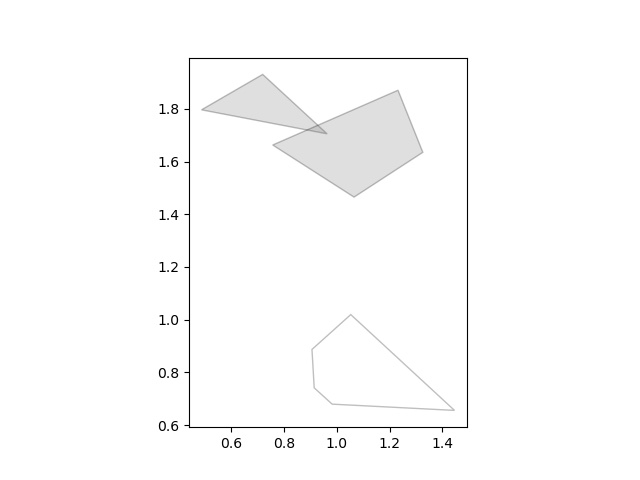
\includegraphics[width= 0.9 \linewidth]{Problem2_scene1.jpg}
	\centering
	\caption{First Scene for Problem 2}
	\label{Problem2_scene1.jpg}
\end{figure}

\begin{figure}[h!]
	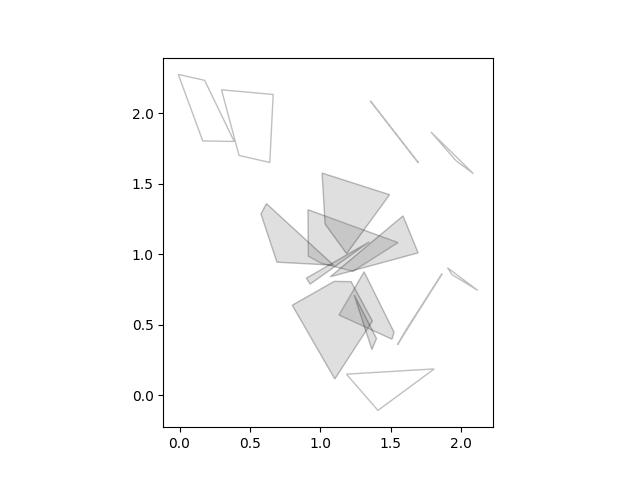
\includegraphics[width= 0.9 \linewidth]{Problem2_scene2.jpg}
	\centering
	\caption{Second Scene for Problem 2}
	\label{Problem2_scene2.jpg}
\end{figure}

\begin{figure}[h!]
	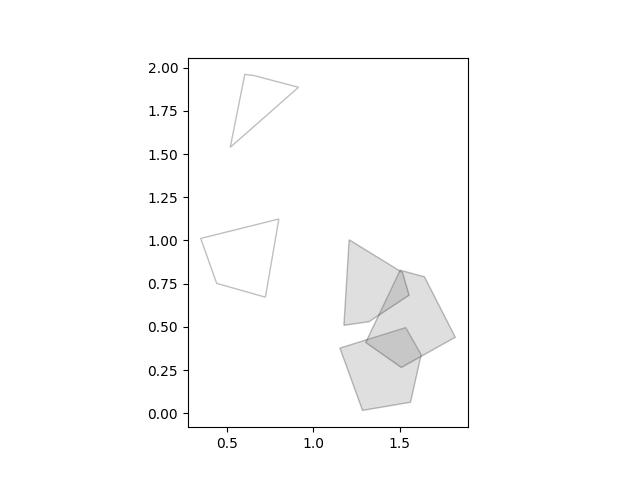
\includegraphics[width= 0.9 \linewidth]{Problem2_scene3.jpg}
	\centering
	\caption{Third Scene for Problem 2}
	\label{Problem2_scene3.jpg}
\end{figure}

\begin{figure}[h!]
	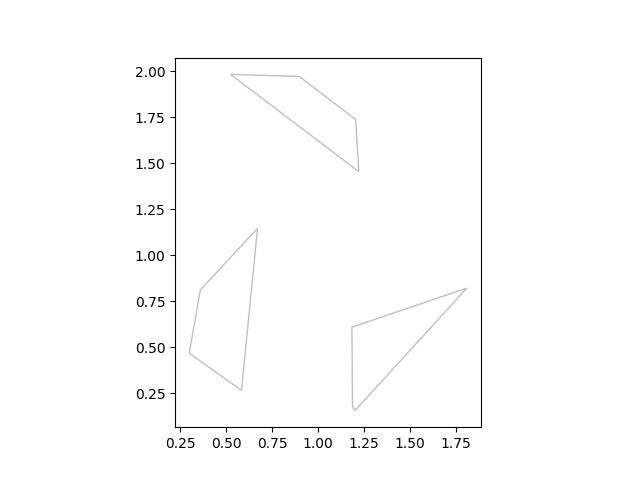
\includegraphics[width= 0.9 \linewidth]{Problem2_scene4.jpg}
	\centering
	\caption{Fourth Scene for Problem 2}
	\label{Problem2_scene4.jpg}
\end{figure}

\begin{figure}[h!]
	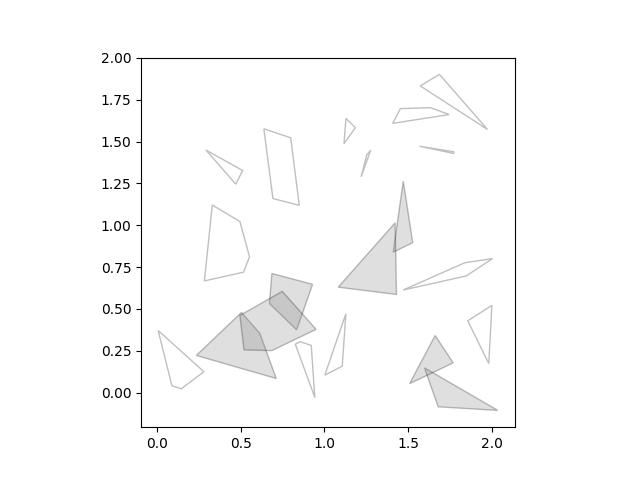
\includegraphics[width= 0.9 \linewidth]{Problem2_scene5.jpg}
	\centering
	\caption{Fifth Scene for Problem 2}
	\label{Problem2_scene5.jpg}
\end{figure}

\begin{figure}[h!]
	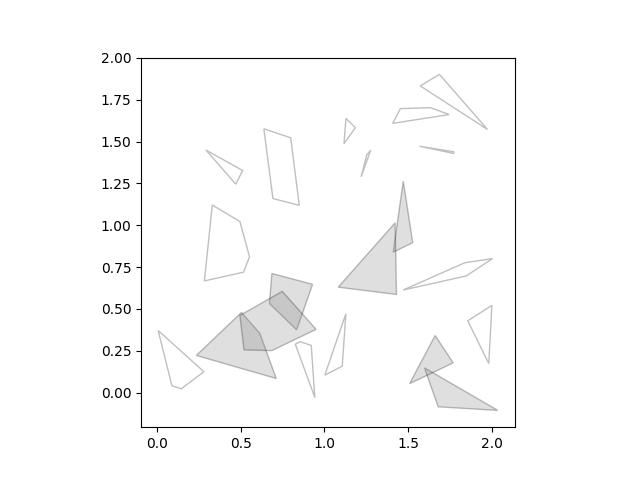
\includegraphics[width= 0.9 \linewidth]{Problem2_scene6.jpg}
	\centering
	\caption{Sixth Scene for Problem 2}
	\label{Problem2_scene6.jpg}
\end{figure}

\begin{figure}[h!]
	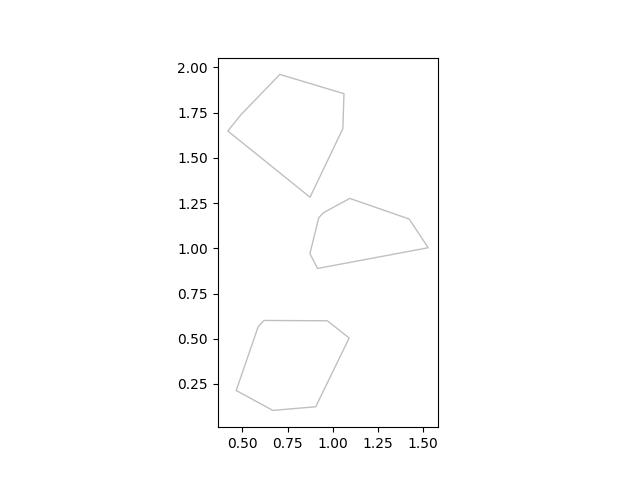
\includegraphics[width= 0.9 \linewidth]{Problem2_scene7.jpg}
	\centering
	\caption{Seventh Scene for Problem 2}
	\label{Problem2_scene7.jpg}
\end{figure}

\begin{figure}[h!]
	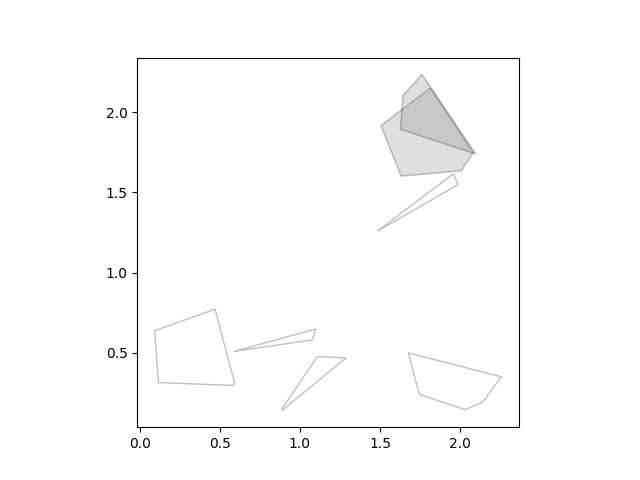
\includegraphics[width= 0.9 \linewidth]{Problem2_scene8.jpg}
	\centering
	\caption{Eighth Scene for Problem 2}
	\label{Problem2_scene8.jpg}
\end{figure}


 
\section{Collision-free Navigation for a 2D rigid body}
 
\section{Collision-free Movement of a Planar Arm}
\subsection{Controlling Planar Arm}
To control the first joint, the up key was for increments and the down key was for decrements. To control the second joint, the right key was for increments and the down key was decrements. The step size was $\pi$/30.
\subsection{Visualization of Scenes}

\begin{figure}[H]
  \centering
  \begin{minipage}{0.45\textwidth}
    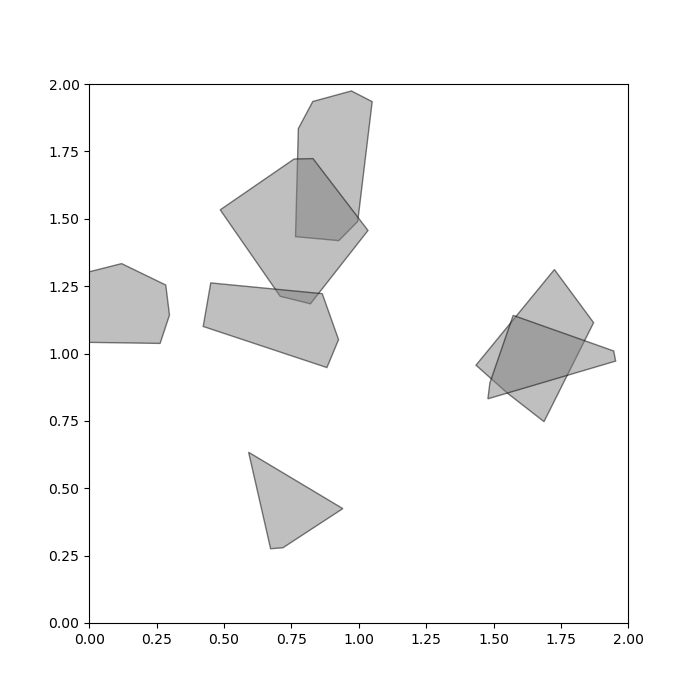
\includegraphics[scale = 0.3]{part4_without_arm.png}
  \end{minipage}\hfill
  \begin{minipage}{0.45\textwidth}
    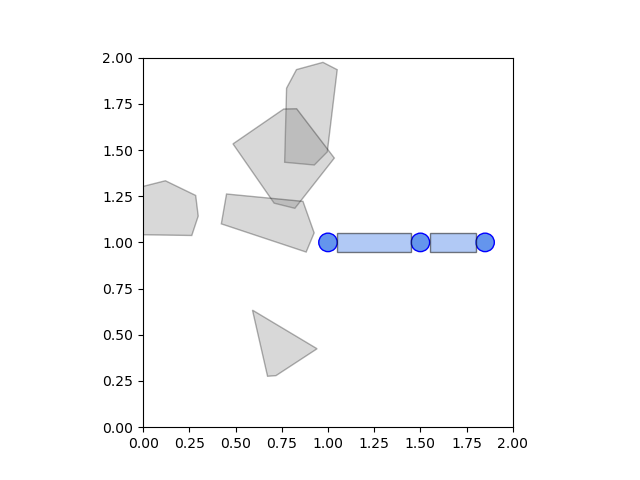
\includegraphics[width=\linewidth]{part4_with_arm.png}
  \end{minipage}
    \caption{Polygons that collide with arm at start are removed}
\end{figure}

\subsection{Collision-Free Configuration Space}
\begin{figure}[htbp]
  \centering
  \begin{minipage}{0.45\textwidth}
    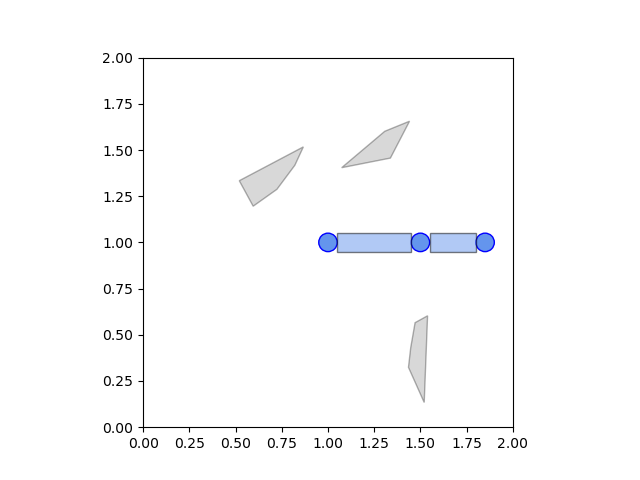
\includegraphics[width=\linewidth]{part4_arm_free.png}
    \caption{Arm collision-free}
  \end{minipage}\hfill
  \begin{minipage}{0.45\textwidth}
    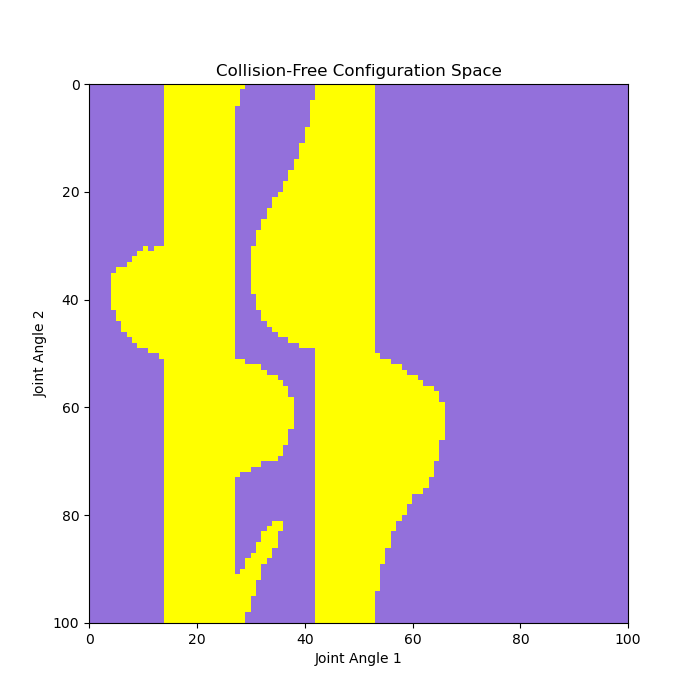
\includegraphics[width=\linewidth]{part4_cspace.png}
    \caption{Configuration Space of fig.15}
  \end{minipage}\hfill
\end{figure}


\end{document}
